% Options for packages loaded elsewhere
\PassOptionsToPackage{unicode}{hyperref}
\PassOptionsToPackage{hyphens}{url}
\PassOptionsToPackage{dvipsnames,svgnames*,x11names*}{xcolor}
%
\documentclass[
  english,
  ,man]{apa6}
\usepackage{lmodern}
\usepackage{amssymb,amsmath}
\usepackage{ifxetex,ifluatex}
\ifnum 0\ifxetex 1\fi\ifluatex 1\fi=0 % if pdftex
  \usepackage[T1]{fontenc}
  \usepackage[utf8]{inputenc}
  \usepackage{textcomp} % provide euro and other symbols
\else % if luatex or xetex
  \usepackage{unicode-math}
  \defaultfontfeatures{Scale=MatchLowercase}
  \defaultfontfeatures[\rmfamily]{Ligatures=TeX,Scale=1}
\fi
% Use upquote if available, for straight quotes in verbatim environments
\IfFileExists{upquote.sty}{\usepackage{upquote}}{}
\IfFileExists{microtype.sty}{% use microtype if available
  \usepackage[]{microtype}
  \UseMicrotypeSet[protrusion]{basicmath} % disable protrusion for tt fonts
}{}
\makeatletter
\@ifundefined{KOMAClassName}{% if non-KOMA class
  \IfFileExists{parskip.sty}{%
    \usepackage{parskip}
  }{% else
    \setlength{\parindent}{0pt}
    \setlength{\parskip}{6pt plus 2pt minus 1pt}}
}{% if KOMA class
  \KOMAoptions{parskip=half}}
\makeatother
\usepackage{xcolor}
\IfFileExists{xurl.sty}{\usepackage{xurl}}{} % add URL line breaks if available
\IfFileExists{bookmark.sty}{\usepackage{bookmark}}{\usepackage{hyperref}}
\hypersetup{
  pdftitle={Supplemental Materials},
  pdfauthor={Brandon LeBeau~\& Ariel M. Aloe},
  pdflang={en-EN},
  pdfkeywords={Research Synthesis, Statistical Software, Quantitative Methods},
  colorlinks=true,
  linkcolor=blue,
  filecolor=Maroon,
  citecolor=Blue,
  urlcolor=Blue,
  pdfcreator={LaTeX via pandoc}}
\urlstyle{same} % disable monospaced font for URLs
\usepackage{longtable,booktabs}
% Correct order of tables after \paragraph or \subparagraph
\usepackage{etoolbox}
\makeatletter
\patchcmd\longtable{\par}{\if@noskipsec\mbox{}\fi\par}{}{}
\makeatother
% Allow footnotes in longtable head/foot
\IfFileExists{footnotehyper.sty}{\usepackage{footnotehyper}}{\usepackage{footnote}}
\makesavenoteenv{longtable}
\usepackage{graphicx,grffile}
\makeatletter
\def\maxwidth{\ifdim\Gin@nat@width>\linewidth\linewidth\else\Gin@nat@width\fi}
\def\maxheight{\ifdim\Gin@nat@height>\textheight\textheight\else\Gin@nat@height\fi}
\makeatother
% Scale images if necessary, so that they will not overflow the page
% margins by default, and it is still possible to overwrite the defaults
% using explicit options in \includegraphics[width, height, ...]{}
\setkeys{Gin}{width=\maxwidth,height=\maxheight,keepaspectratio}
% Set default figure placement to htbp
\makeatletter
\def\fps@figure{htbp}
\makeatother
\setlength{\emergencystretch}{3em} % prevent overfull lines
\providecommand{\tightlist}{%
  \setlength{\itemsep}{0pt}\setlength{\parskip}{0pt}}
\setcounter{secnumdepth}{-\maxdimen} % remove section numbering
\shorttitle{Supplemental Materials}
\affiliation{
\vspace{0.5cm}
\textsuperscript{1} University of Iowa}
\keywords{Research Synthesis, Statistical Software, Quantitative Methods}
\usepackage{csquotes}
\usepackage{upgreek}
\captionsetup{font=singlespacing,justification=justified}

\usepackage{longtable}
\usepackage{lscape}
\usepackage{multirow}
\usepackage{tabularx}
\usepackage[flushleft]{threeparttable}
\usepackage{threeparttablex}

\newenvironment{lltable}{\begin{landscape}\begin{center}\begin{ThreePartTable}}{\end{ThreePartTable}\end{center}\end{landscape}}

\makeatletter
\newcommand\LastLTentrywidth{1em}
\newlength\longtablewidth
\setlength{\longtablewidth}{1in}
\newcommand{\getlongtablewidth}{\begingroup \ifcsname LT@\roman{LT@tables}\endcsname \global\longtablewidth=0pt \renewcommand{\LT@entry}[2]{\global\advance\longtablewidth by ##2\relax\gdef\LastLTentrywidth{##2}}\@nameuse{LT@\roman{LT@tables}} \fi \endgroup}


\DeclareDelayedFloatFlavor{ThreePartTable}{table}
\DeclareDelayedFloatFlavor{lltable}{table}
\DeclareDelayedFloatFlavor*{longtable}{table}
\makeatletter
\renewcommand{\efloat@iwrite}[1]{\immediate\expandafter\protected@write\csname efloat@post#1\endcsname{}}
\makeatother
\usepackage{tabularx}
\usepackage{pdflscape}
\ifxetex
  % Load polyglossia as late as possible: uses bidi with RTL langages (e.g. Hebrew, Arabic)
  \usepackage{polyglossia}
  \setmainlanguage[]{english}
\else
  \usepackage[shorthands=off,main=english]{babel}
\fi

\title{Supplemental Materials}
\author{Brandon LeBeau\textsuperscript{1}~\& Ariel M. Aloe\textsuperscript{1}}
\date{}

\authornote{

Correspondence concerning this article should be addressed to Brandon LeBeau, Psychological and Quantitative Foundations, University of Iowa, Iowa City, IA 52245. E-mail: \href{mailto:brandon-lebeau@uiowa.edu}{\nolinkurl{brandon-lebeau@uiowa.edu}}}

\abstract{
Statistical software is the enabling tool of quantitative research and the availability and use of the software can greatly shape which methods are used by researchers. Software that is more accessible is likely to have more users and the methods implemented within the software limits the methods accessible to researchers. Open source software, (e.g.~R), has reduced these barriers by making cutting edge statistical methods available to researchers through add-on packages. This manuscript explores the evolution of statistical software within social science research using a research synthesis to establish the state of affairs.


}

\begin{document}
\maketitle

\begin{figure}
\centering
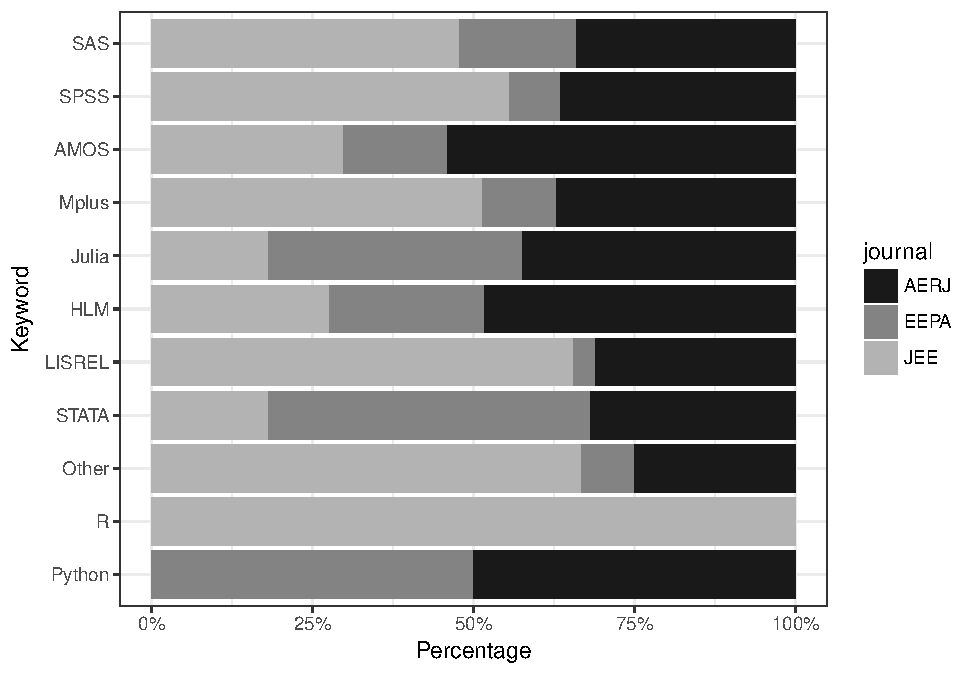
\includegraphics{supplemental_files/figure-latex/software-journal-1.pdf}
\caption{\label{fig:software-journal}Software counts by journal}
\end{figure}

Expanding on the software keywords found within the PDFs, Figure \ref{fig:software-journal} explores which software keywords were found in each journal. In general, mirroring results from Figure \ref{fig:count-software}, the percentage of articles reporting software keywords was relatively small, most often less than 5\%. R, SAS, SPSS, and Stata were the most commonly found software keywords, with R being the most common in most journals. The one exception to this was in JEE, where SAS was more common (about 20\% of articles), with R and SPSS having a similar percentage (about 15\%) of articles reporting their usage. One interpretation note, articles may mention more than one software keyword and those duplicate results will show up in each category. On average, the average number of software keywords identified in each article was highest for JEE at 1.71 (range: 1 to 5) and a lowest of 1 for PPA (range: 1 to 1).

A similar figure for model keywords can be seen in Figure \ref{fig:model-journal}. The x-axis scale here is wider compared to the software keywords showing that the methods are more commonly reported. However, there are still a sizable number of articles appearing in these journals that do not list one of the model keywords searched. The most commonly used methods are linear model, analysis of variance, meta-analysis, or linear mixed (i.e.~HLM or multilevel) models. The journals EEPA, JEE, and SE have the widest array of models identified through the keyword search. On the opposite side, AEJ, AJPS, and EJ are dominated by linear models. Finally, journals such as AERJ, ER, HE, PPA, and PSQ all have a low prevalence of articles that are using the model keywords.

\begin{figure}
\centering
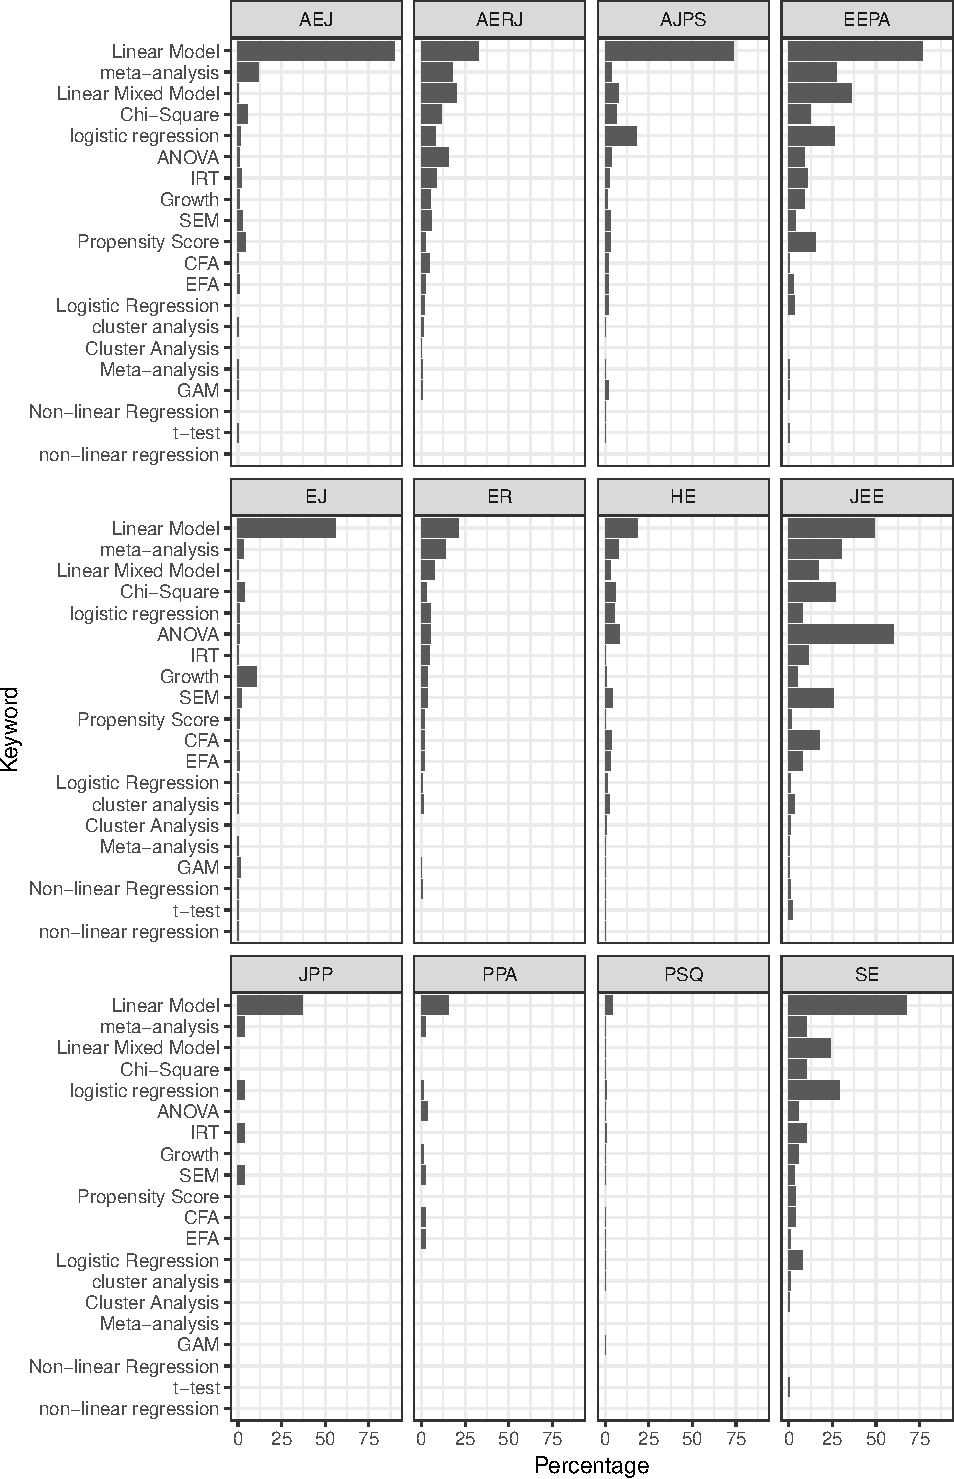
\includegraphics{supplemental_files/figure-latex/model-journal-1.pdf}
\caption{\label{fig:model-journal}Statistical Model counts by journal}
\end{figure}

\hypertarget{impact-of-publication-year-on-keyword-rates}{%
\subsection{Impact of publication year on keyword rates}\label{impact-of-publication-year-on-keyword-rates}}

The impact of publication year on prevalence of software and model keywords was explored in Figures \ref{fig:software-year-at1} and \ref{fig:model-year-at1} for common software and model keywords respectively. In general, publication year does not have a strong impact on the software keyword rates with most trajectories being flat across the publication years. The one exception to this is with SAS which on average has declined across the publication years. R has consistently been the most cited software across these publication years for these journals, but overall software was infrequently cited (see Figure \ref{fig:software-journal}).

Commonly used specialty software, such as AMOS, HLM, LISREL, or Mplus, are shown in the bottom-most plot of Figure \ref{fig:software-year-at1}. Not surprisingly, the specialty software on average shows up less frequently compared to the general purpose software shown in the top-most plot of Figure \ref{fig:software-year-at1}. Out of these four specialty software, AMOS tends to be used the most frequently, LISREL has decreased in usage since 1995, and Mplus has gained additional usage. However, these programs still only account for around 10\% or less of statistical software used.

The usage of model keywords occurs more frequently and shows evidence of trends across publication years as shown in Figure \ref{fig:model-year-at1}. For example, the top figure shows a large increase in the prevalence of terms related to linear models (i.e.~regression models) or linear mixed models and shows a decline in analysis of variance methods. Logistic regression and the variety of t-tests are rarely mentioned in the articles included. The bottom figure also shows general increases in the four models depicted, particularly the mention of IRT and SEM methods. These gains are more modest compared to the increase in the mention of linear models from the top figure, but the increase has now put IRT and SEM methods about the same percentage as ANOVA from the top figure.

\hypertarget{interaction-between-software-and-statistical-methods}{%
\subsection{Interaction between software and statistical methods}\label{interaction-between-software-and-statistical-methods}}

Figure \ref{fig:software-statmethods} shows a tile plot of the interaction between software (x-axis) and model (y-axis) keywords. The darker shaded regions of the figure show more combinations of the software and model keywords. In the figure, publication year is ignored to identify which methods are most closely paired with specific software. There are duplicates in the data for this figure, for example, an article may cite both R and SAS within the document and mentioned using a linear model. In this case, this article will show up in the R/linear model cell as well as the SAS/linear model cell. Any duplicate keyword combinations would only occur once for each article. This analysis is also limited to articles that have both a software and model keyword returned. On average, only about 20\% of all the PDFs obtained from the study had both a software and model keyword in them. This provides further evidence of the reporting bias, particularly with regard to software.

The figure shows that the two most common combinations are R and ANOVA and SAS and linear model. ANOVA is also common with more specialized software such as AMOS, LISREL, or Mplus that may indicate these are being used for nested model comparisons. Linear mixed models were most commonly used in SAS, with R and HLM software being the next highest percentages. Meta-analysis is most commonly associated with SPSS. Interestingly, IRT models are associated with R more than specialized IRT software, however the number of articles using IRT may be quite small and may not adequately cite the software used.

The impact of publication year is explored next for the four general purpose statistical software, R, SAS, SPSS, and Stata. In addition, the models explored were restricted to reflect more general purpose statistical procedures. Each panel in Figure \ref{fig:software-statmethods-year} represents a different publication year. In the panel label the percentage of articles that are missing. More specifically, these are studies in which a PDF document was obtained but did not include software and model keyword. These values range from a low of 70\% of the articles not appearing to a high of about 88\%. The percentage of missing articles does decrease slightly in recent years, however there is still evidence of reporting bias.

The tile plot shown in Figure \ref{fig:software-statmethods-year} shows an increase in the percentage of keyword combinations that are found as the publications become more recent. This is particularly true for R, SAS, and SPSS software regardless of the model used. On the other hand, Stata appears infrequently within each year, but there is evidence of Stata appearing more frequently with more recent publications. There does not appear to be any significant trends over time with regard to which models are used in particular software, but there were articles using R, SAS, and SPSS with most of the statistical models shown in Figure \ref{fig:software-statmethods-year} which supports the general usage of the software across a variety of model situations.

\begin{figure}
\centering
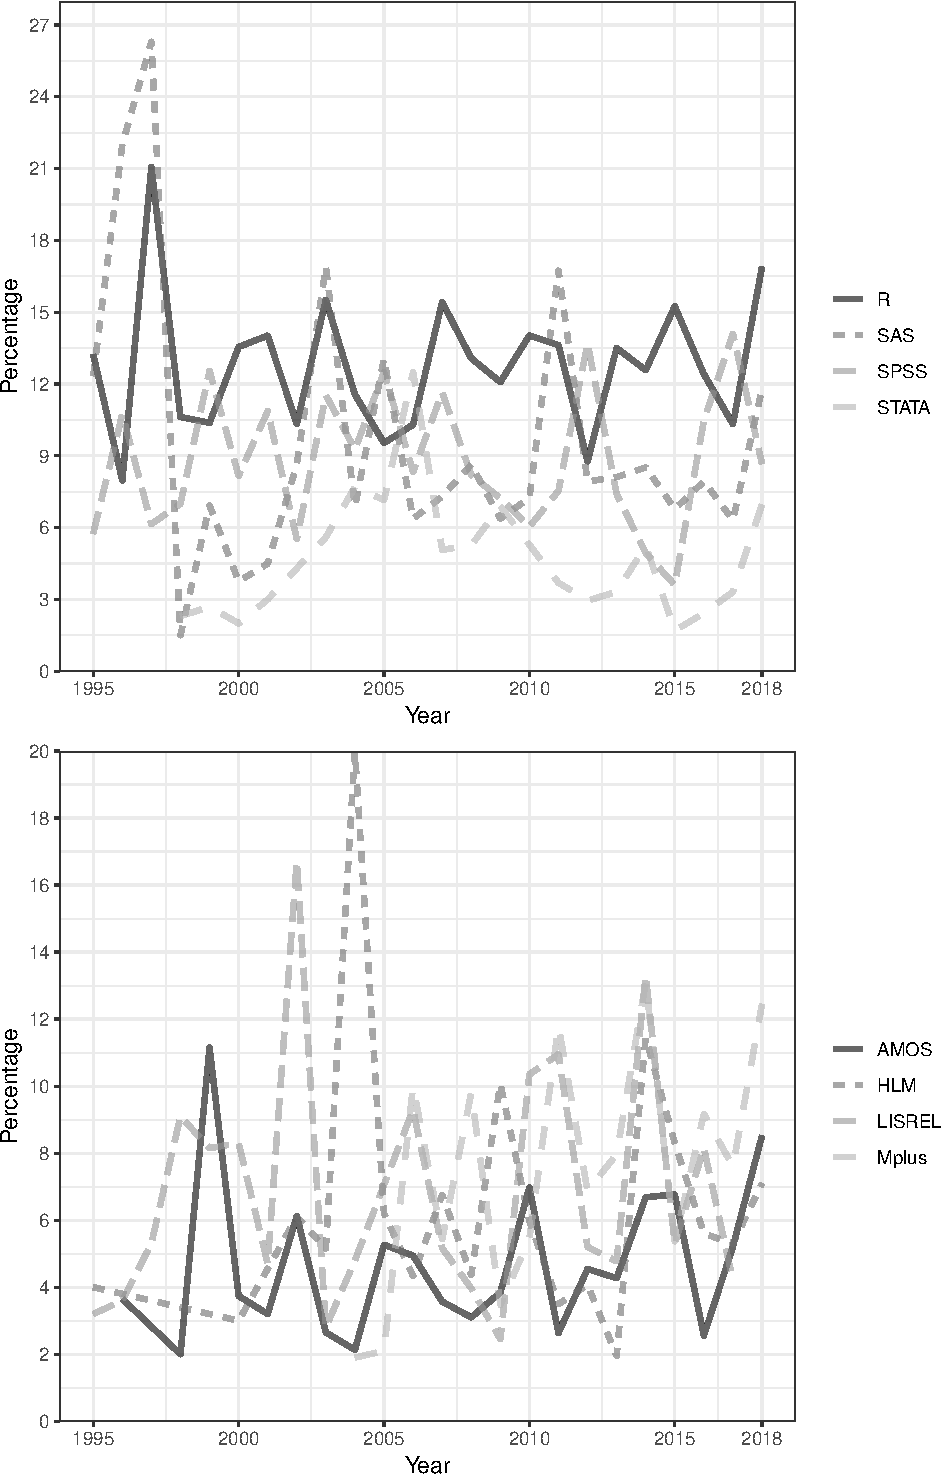
\includegraphics{supplemental_files/figure-latex/software-year-at1-1.pdf}
\caption{\label{fig:software-year-at1}Software percentages by year}
\end{figure}

\begin{figure}
\centering
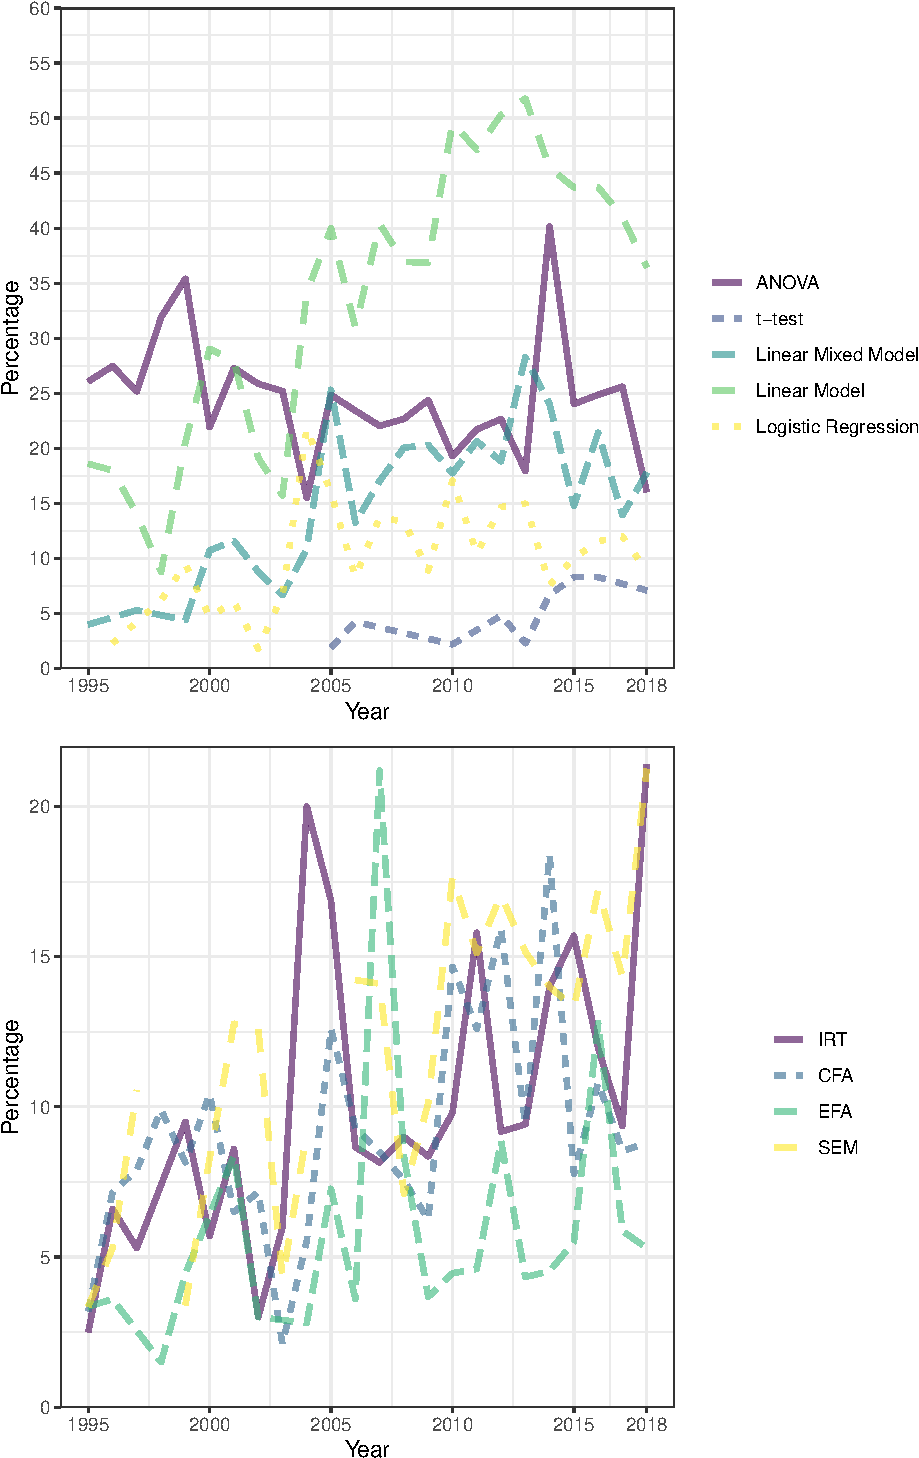
\includegraphics{supplemental_files/figure-latex/model-year-at1-1.pdf}
\caption{\label{fig:model-year-at1}Model percentages by year}
\end{figure}

\begin{figure}
\centering
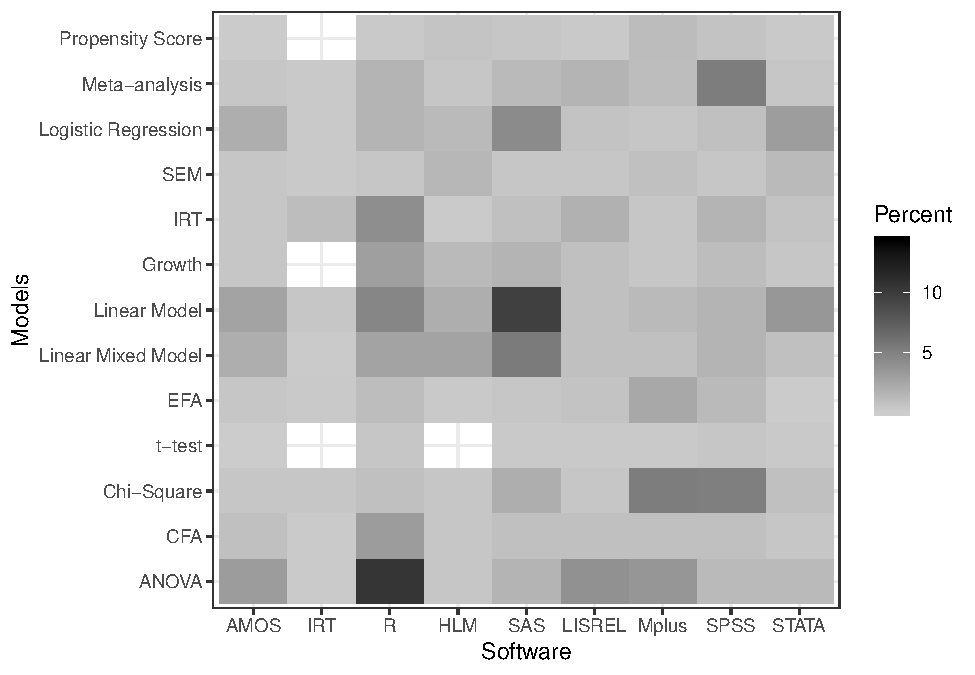
\includegraphics{supplemental_files/figure-latex/software-statmethods-1.pdf}
\caption{\label{fig:software-statmethods}Tile plot showing interaction between software and statistical methods.}
\end{figure}

\begin{figure}
\centering
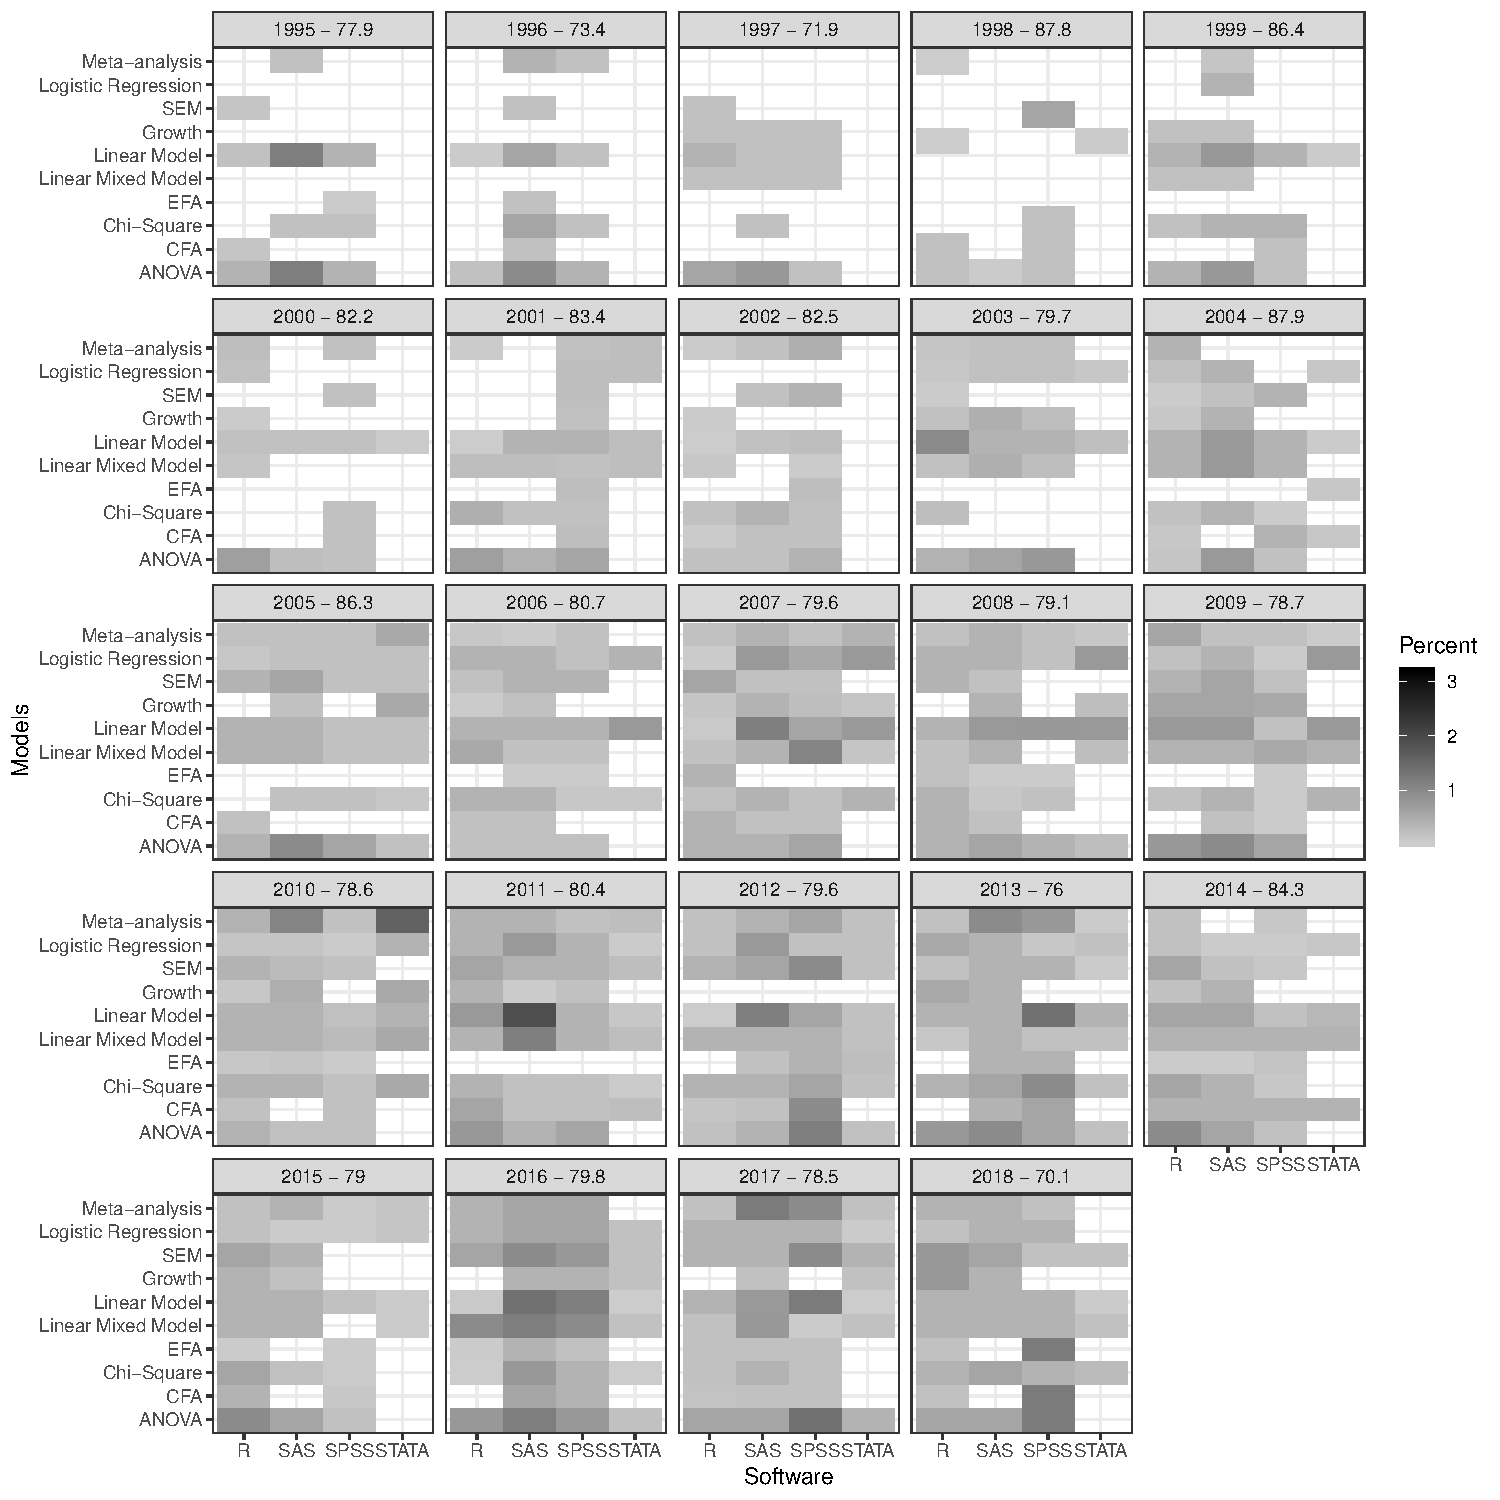
\includegraphics{supplemental_files/figure-latex/software-statmethods-year-1.pdf}
\caption{\label{fig:software-statmethods-year}Tile plot showing interaction between software and statistical methods by publication year for primary software.}
\end{figure}

\end{document}
